\chapter{\protect\hyperlink{:}{电磁学}}
\addtocontents{toc}{\protect\hypertarget{:}{}}


\section{\protect\hyperlink{:}{静电场、稳恒电流}}
\addtocontents{toc}{\protect\hypertarget{:}{}}


\subsection{\protect\hyperlink{:}{静电场的基本规律}}
\addtocontents{toc}{\protect\hypertarget{:}{}}

\subsubsection{\protect\hyperlink{:}{库仑定律}}
\addtocontents{toc}{\protect\hypertarget{:}{}}

静电学的基础始于对点电荷之间相互作用力的描述。库仑通过扭秤实验总结出了两个静止点电荷之间的作用力规律。

\begin{theorem}[库仑定律]
    在真空中，两个静止点电荷之间的相互作用力的大小与它们的电荷量的乘积成正比，与它们之间距离的平方成反比，方向沿着两点电荷连线，同号相斥、异号相吸：
    \begin{equation}
        \vec{F}_{12} = \frac{1}{4\pi\varepsilon_0}\frac{q_1 q_2}{r_{12}^2}\hat{r}_{12}
    \end{equation}
    其中 $\varepsilon_0 = 8.854 \times 10^{-12}$ C$^2$/(N$\cdot$m$^2$) 为真空介电常量，$\hat{r}_{12}$ 是从 $q_1$ 指向 $q_2$ 的单位矢量。
\end{theorem}

\begin{remark}
    库仑定律的适用条件：(1) 真空中；(2) 静止的点电荷。对于不能简化为点电荷的带电体，需要将其分割为无穷多个电荷微元，再利用叠加原理求解。
\end{remark}

\subsubsection{\protect\hyperlink{:}{电场强度与叠加原理}}
\addtocontents{toc}{\protect\hypertarget{:}{}}

电荷之间的相互作用是通过\textbf{电场}来传递的。为了描述电场的性质，我们引入电场强度的概念。

\begin{definition}[电场强度]
    在空间某点放入一个试探电荷 $q_0$（要求足够小，不扰动原电场），其所受的电场力 $\vec{F}$ 与试探电荷电量 $q_0$ 的比值定义为该点的电场强度
    \begin{equation}
        \vec{E} = \frac{\vec{F}}{q_0}
    \end{equation}
    电场强度是矢量，其方向为正试探电荷在该点所受力的方向。
\end{definition}

一个点电荷 $q$ 在距离 $r$ 处产生的电场强度为
\begin{equation}
    \vec{E} = \frac{1}{4\pi\varepsilon_0}\frac{q}{r^2}\hat{r}
\end{equation}

\begin{theorem}[场强叠加原理]
    多个点电荷在空间某点产生的合电场强度等于各点电荷单独存在时在该点产生的电场强度的矢量和
    \begin{equation}
        \vec{E} = \sum_i \vec{E}_i = \frac{1}{4\pi\varepsilon_0}\sum_i \frac{q_i}{r_i^2}\hat{r}_i
    \end{equation}
    对于连续分布的电荷，求和替换为积分
    \begin{equation}
        \vec{E} = \frac{1}{4\pi\varepsilon_0}\int \frac{\mathrm{d}q}{r^2}\hat{r}
    \end{equation}
\end{theorem}

\subsubsection{\protect\hyperlink{:}{电偶极子}}
\addtocontents{toc}{\protect\hypertarget{:}{}}

电偶极子是电学中一个非常重要的模型，它由两个等量异号的点电荷 $+q$ 和 $-q$ 组成，间距为 $l$。

\begin{definition}[电偶极子与电偶极矩]
    电偶极矩定义为
    \begin{equation}
        \vec{p} = q\vec{l}
    \end{equation}
    其中 $\vec{l}$ 是从负电荷指向正电荷的矢量。电偶极矩是描述电偶极子特性的核心物理量。
\end{definition}

\begin{example}[电偶极子的电场]
    求电偶极子在连接线延长线上以及中垂线上的电场强度。
    \begin{figure}[hbtp]
        \centering
        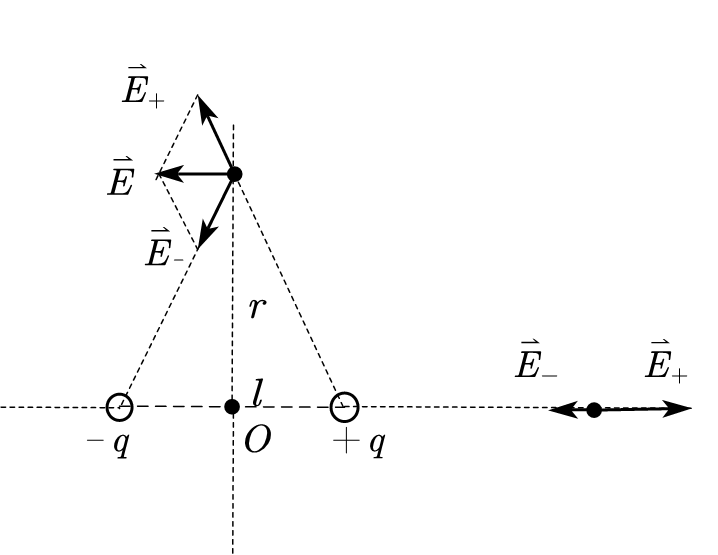
\includegraphics[width=0.4\textwidth]{figure/电偶极子.png}
        \caption{电偶极子}
        \label{fig:电偶极子}
    \end{figure}
    
    \begin{solution}
        \textbf{延长线上}：设场点距离偶极子中心 $r$（$r \gg l$），则正负电荷产生的电场分别为
        \begin{equation}
            E_+ = \frac{1}{4\pi\varepsilon_0}\frac{q}{(r-l/2)^2}, \qquad E_- = \frac{1}{4\pi\varepsilon_0}\frac{q}{(r+l/2)^2}
        \end{equation}
        两者方向相反，合场强为（取 $r \gg l$ 的近似）
        \begin{equation}
            E_{\text{延长线}} = E_+ - E_- \approx \frac{1}{4\pi\varepsilon_0}\frac{2ql}{r^3} = \frac{1}{4\pi\varepsilon_0}\frac{2p}{r^3}
        \end{equation}

        \textbf{中垂线上}：设场点距离偶极子中心 $r$，两个电荷产生的电场大小相等，竖直分量相互抵消，水平分量叠加
        \begin{equation}
            E_{\text{中垂线}} = 2E_+\cos\theta \approx \frac{1}{4\pi\varepsilon_0}\frac{ql}{r^3} = \frac{1}{4\pi\varepsilon_0}\frac{p}{r^3}
        \end{equation}
        其中 $\cos\theta = l/(2\sqrt{r^2+l^2/4}) \approx l/(2r)$。
    \end{solution}

    \begin{remark}
        电偶极子的电场随距离以 $1/r^3$ 衰减，比点电荷的 $1/r^2$ 更快。这是因为正负电荷的贡献在远处几乎抵消，只剩下偶极矩的贡献。
    \end{remark}
\end{example}

\subsubsection{\protect\hyperlink{:}{高斯定理}}
\addtocontents{toc}{\protect\hypertarget{:}{}}

高斯定理是静电学中最重要的定理之一，它揭示了电场与电荷之间的深层联系。

\begin{definition}[电通量]
    通过一个面元 $\mathrm{d}\vec{S}$ 的电通量定义为
    \begin{equation}
        \mathrm{d}\Phi_E = \vec{E} \cdot \mathrm{d}\vec{S} = E\cos\theta\,\mathrm{d}S
    \end{equation}
    通过一个有限曲面 $S$ 的电通量为
    \begin{equation}
        \Phi_E = \iint_S \vec{E} \cdot \mathrm{d}\vec{S}
    \end{equation}
\end{definition}

\begin{theorem}[高斯定理]
    通过任意闭合曲面 $S$ 的电通量等于该闭合曲面所包围的净电荷量除以 $\varepsilon_0$
    \begin{equation}
        \oiint_S \vec{E} \cdot \mathrm{d}\vec{S} = \frac{Q_{\text{内}}}{\varepsilon_0}
    \end{equation}
    其中 $Q_{\text{内}}$ 是闭合曲面内的总电荷量。
\end{theorem}

高斯定理的证明思路：对于单个点电荷，以它为球心作半径为 $r$ 的球面，通过球面的电通量为
\begin{equation}
    \Phi_E = \oiint_S \vec{E} \cdot \mathrm{d}\vec{S} = \frac{q}{4\pi\varepsilon_0 r^2}\cdot 4\pi r^2 = \frac{q}{\varepsilon_0}
\end{equation}

由于电通量与球面半径无关，对于任意闭合曲面，只要点电荷在曲面内部，通过的电通量都是 $q/\varepsilon_0$。再利用叠加原理，即可得到一般形式的高斯定理。

高斯定理的一个重要应用是计算具有高度对称性的电荷分布的电场。选择合适的高斯面，使得电场在面上为常量或为零，就可以方便地求出电场。

\begin{example}[无限大均匀带电平面的电场]
    设电荷面密度为 $\sigma$，由对称性，电场方向垂直于平面，大小只与到平面的距离有关。作圆柱形高斯面，两底面平行于带电平面
    \begin{equation}
        \oiint_S \vec{E} \cdot \mathrm{d}\vec{S} = 2EA = \frac{\sigma A}{\varepsilon_0}
    \end{equation}
    解得
    \begin{equation}
        E = \frac{\sigma}{2\varepsilon_0}
    \end{equation}
    电场是匀强的，与距离无关。
\end{example}

\subsubsection{\protect\hyperlink{:}{电势}}
\addtocontents{toc}{\protect\hypertarget{:}{}}

由于静电场力是保守力（$\nabla \times \vec{E} = \vec{0}$），我们可以引入电势的概念。

\begin{definition}[电势]
    空间中 $A$ 点与 $B$ 点之间的电势差定义为将单位正电荷从 $A$ 移到 $B$ 时电场力所做的功
    \begin{equation}
        V_A - V_B = \int_A^B \vec{E} \cdot \mathrm{d}\vec{l}
    \end{equation}
    通常选取无穷远处为电势零点（$V_\infty = 0$），则 $A$ 点的电势为
    \begin{equation}
        V_A = \int_A^\infty \vec{E} \cdot \mathrm{d}\vec{l}
    \end{equation}
\end{definition}

对于点电荷 $q$，距离 $r$ 处的电势为
\begin{equation}
    V = \frac{1}{4\pi\varepsilon_0}\frac{q}{r}
\end{equation}

电势满足叠加原理：多个点电荷在某点产生的电势等于各点电荷单独存在时在该点产生的电势的代数和（标量叠加，比矢量叠加简单得多）。

电场强度与电势的关系为
\begin{equation}
    \vec{E} = -\nabla V = -\left(\frac{\partial V}{\partial x}\hat{i} + \frac{\partial V}{\partial y}\hat{j} + \frac{\partial V}{\partial z}\hat{k}\right)
\end{equation}

\subsubsection{\protect\hyperlink{:}{静电场的环路定理}}
\addtocontents{toc}{\protect\hypertarget{:}{}}

\begin{theorem}[静电场的环路定理]
    静电场沿任意闭合路径的环量为零
    \begin{equation}
        \oint \vec{E} \cdot \mathrm{d}\vec{l} = 0
    \end{equation}
    这等价于说静电场是无旋场（$\nabla \times \vec{E} = \vec{0}$），也等价于静电力是保守力。
\end{theorem}

环路定理和高斯定理一起，完整地描述了静电场的性质：高斯定理描述电场的"源"（有源性），环路定理描述电场的"旋"（无旋性）。


\subsection{\protect\hyperlink{:}{稳恒电流}}
\addtocontents{toc}{\protect\hypertarget{:}{}}

\subsubsection{\protect\hyperlink{:}{电流与电流密度}}
\addtocontents{toc}{\protect\hypertarget{:}{}}

电荷的定向移动形成\textbf{电流}。为了描述电流的分布，我们引入电流密度的概念。

\begin{definition}[电流强度]
    通过某截面的电流强度定义为单位时间内通过该截面的电荷量
    \begin{equation}
        I = \frac{\mathrm{d}q}{\mathrm{d}t}
    \end{equation}
\end{definition}

\begin{definition}[电流密度]
    电流密度 $\vec{j}$ 是一个矢量，其方向为正电荷的漂移方向，大小等于单位时间通过垂直于电流方向的单位面积的电荷量
    \begin{equation}
        \vec{j} = nq\vec{v}_d
    \end{equation}
    其中 $n$ 为载流子数密度，$q$ 为载流子电荷量，$\vec{v}_d$ 为漂移速度。
\end{definition}

电流强度与电流密度的关系为
\begin{equation}
    I = \iint_S \vec{j} \cdot \mathrm{d}\vec{S}
\end{equation}

\subsubsection{\protect\hyperlink{:}{欧姆定律的微分形式}}
\addtocontents{toc}{\protect\hypertarget{:}{}}

欧姆定律的宏观形式 $U = IR$ 可以推广为微分形式
\begin{equation}
    \vec{j} = \sigma\vec{E}
\end{equation}

其中 $\sigma$ 为材料的电导率。这是描述导体内部电流与电场关系的基本方程。

\subsubsection{\protect\hyperlink{:}{稳恒电流的连续性方程}}
\addtocontents{toc}{\protect\hypertarget{:}{}}

由电荷守恒，流出一个闭合曲面的电流等于曲面内电荷的减少率
\begin{equation}
    \oiint_S \vec{j} \cdot \mathrm{d}\vec{S} = -\frac{\mathrm{d}q}{\mathrm{d}t}
\end{equation}

对于稳恒电流（$\frac{\partial \rho}{\partial t} = 0$），上式变为
\begin{equation}
    \oiint_S \vec{j} \cdot \mathrm{d}\vec{S} = 0
\end{equation}

这意味着在稳恒电流条件下，流入任意闭合曲面的电流等于流出的电流——电流是连续的，不会在某处"堆积"。


\newpage
\section{\protect\hyperlink{:}{恒磁场}}
\addtocontents{toc}{\protect\hypertarget{:}{}}

\subsection{\protect\hyperlink{:}{磁场的基本规律}}
\addtocontents{toc}{\protect\hypertarget{:}{}}

\subsubsection{\protect\hyperlink{:}{磁感应强度}}
\addtocontents{toc}{\protect\hypertarget{:}{}}

运动的电荷（电流）在其周围空间产生\textbf{磁场}。为了描述磁场的强弱和方向，我们引入磁感应强度 $\vec{B}$。

\begin{definition}[磁感应强度]
    一个运动的试探电荷 $q_0$ 以速度 $\vec{v}$ 通过空间某点时，受到的磁力为
    \begin{equation}
        \vec{F} = q_0\vec{v} \times \vec{B}
    \end{equation}
    由此定义该点的磁感应强度 $\vec{B}$。$\vec{B}$ 的方向沿试探电荷不受力的方向（即 $\vec{v}$ 的方向），$\vec{B}$ 的大小为
    \begin{equation}
        B = \frac{F_{\max}}{q_0 v}
    \end{equation}
    其中 $F_{\max}$ 是试探电荷受到的最大磁力。
\end{definition}

\subsubsection{\protect\hyperlink{:}{毕奥-萨伐尔定律}}
\addtocontents{toc}{\protect\hypertarget{:}{}}

电流元 $I\mathrm{d}\vec{l}$ 在空间某点产生的磁感应强度由\textbf{毕奥-萨伐尔定律}给出。

\begin{theorem}[毕奥-萨伐尔定律]
    电流元 $I\mathrm{d}\vec{l}$ 在距离 $\vec{r}$ 处产生的磁感应强度为
    \begin{equation}
        \mathrm{d}\vec{B} = \frac{\mu_0}{4\pi}\frac{I\mathrm{d}\vec{l} \times \hat{r}}{r^2}
    \end{equation}
    其中 $\mu_0 = 4\pi \times 10^{-7}$ T$\cdot$m/A 为真空磁导率，$\hat{r}$ 是从电流元指向场点的单位矢量。
\end{theorem}

对于一个完整的载流导线，总磁感应强度为所有电流元贡献的叠加
\begin{equation}
    \vec{B} = \frac{\mu_0}{4\pi}\int \frac{I\mathrm{d}\vec{l} \times \hat{r}}{r^2}
\end{equation}

\begin{example}[无限长直导线的磁场]
    设导线中电流为 $I$，场点到导线的垂直距离为 $a$。由毕奥-萨伐尔定律积分可得
    \begin{equation}
        B = \frac{\mu_0 I}{2\pi a}
    \end{equation}
    磁场方向沿以导线为轴的圆周的切线方向（右手定则）。
\end{example}

\begin{example}[圆形电流中心的磁场]
    设半径为 $R$ 的圆环中通有电流 $I$，则圆心处的磁感应强度为
    \begin{equation}
        B = \frac{\mu_0 I}{2R}
    \end{equation}
\end{example}

\subsubsection{\protect\hyperlink{:}{磁场的高斯定理}}
\addtocontents{toc}{\protect\hypertarget{:}{}}

\begin{theorem}[磁场的高斯定理]
    通过任意闭合曲面的磁通量恒为零
    \begin{equation}
        \oiint_S \vec{B} \cdot \mathrm{d}\vec{S} = 0
    \end{equation}
    这意味着不存在磁单极子——磁力线总是闭合的，没有起点和终点。
\end{theorem}

\subsubsection{\protect\hyperlink{:}{安培环路定理}}
\addtocontents{toc}{\protect\hypertarget{:}{}}

\begin{theorem}[安培环路定理]
    磁感应强度沿任意闭合路径的环量等于该路径所包围的电流的 $\mu_0$ 倍
    \begin{equation}
        \oint \vec{B} \cdot \mathrm{d}\vec{l} = \mu_0 I_{\text{内}}
    \end{equation}
    其中 $I_{\text{内}}$ 是穿过以闭合路径为边界的曲面的净电流。
\end{theorem}

安培环路定理在计算具有高度对称性的电流分布的磁场时非常有用。

\begin{example}[螺线管内的磁场]
    设螺线管单位长度匝数为 $n$，电流为 $I$。作矩形安培环路，一边在管内、一边在管外。由于管外磁场近似为零，可得
    \begin{equation}
        B = \mu_0 n I
    \end{equation}
    螺线管内部为均匀磁场。
\end{example}

\subsection{\protect\hyperlink{:}{磁场对电流的作用}}
\addtocontents{toc}{\protect\hypertarget{:}{}}

\subsubsection{\protect\hyperlink{:}{安培力}}
\addtocontents{toc}{\protect\hypertarget{:}{}}

磁场对载流导线有力的作用，这个力称为\textbf{安培力}。

\begin{theorem}[安培力公式]
    电流元 $I\mathrm{d}\vec{l}$ 在磁场 $\vec{B}$ 中受到的安培力为
    \begin{equation}
        \mathrm{d}\vec{F} = I\mathrm{d}\vec{l} \times \vec{B}
    \end{equation}
\end{theorem}

\subsubsection{\protect\hyperlink{:}{磁矩与磁力矩}}
\addtocontents{toc}{\protect\hypertarget{:}{}}

\begin{definition}[磁矩]
    一个面积为 $S$、电流为 $I$ 的平面线圈的磁矩定义为
    \begin{equation}
        \vec{m} = IS\hat{n}
    \end{equation}
    其中 $\hat{n}$ 为线圈平面的法向量（由右手定则确定）。
\end{definition}

在均匀磁场中，一个载流线圈受到的合力为零，但受到一个力矩
\begin{equation}
    \vec{M} = \vec{m} \times \vec{B}
\end{equation}

这个力矩使线圈的磁矩趋向于与外磁场方向一致。这正是电动机的工作原理。


\newpage
\section{\protect\hyperlink{:}{电磁感应}}
\addtocontents{toc}{\protect\hypertarget{:}{}}

\subsection{\protect\hyperlink{:}{法拉第电磁感应定律}}
\addtocontents{toc}{\protect\hypertarget{:}{}}

法拉第通过实验发现，变化的磁场可以产生电场——这是电磁学中最重要的发现之一。

\begin{theorem}[法拉第电磁感应定律]
    当通过一个闭合回路的磁通量发生变化时，回路中将产生感应电动势
    \begin{equation}
        \mathcal{E} = -\frac{\mathrm{d}\Phi_B}{\mathrm{d}t}
    \end{equation}
    其中 $\Phi_B = \iint_S \vec{B} \cdot \mathrm{d}\vec{S}$ 是通过回路的磁通量。负号表示感应电动势的方向遵循\textbf{楞次定律}：感应电流产生的磁场总是阻碍引起感应的磁通量变化。
\end{theorem}

磁通量变化的原因可以有多种：
\begin{enumerate}
    \item 磁场随时间变化（$\partial \vec{B}/\partial t \neq 0$）
    \item 回路面积变化（如导体棒在磁场中滑动）
    \item 回路与磁场的夹角变化（如线圈在磁场中旋转）
\end{enumerate}

\begin{example}[导体棒在磁场中滑动]
    一根长为 $L$ 的导体棒在垂直于均匀磁场 $\vec{B}$ 的平面内以速度 $\vec{v}$ 滑动。棒两端产生的动生电动势为
    \begin{equation}
        \mathcal{E} = BLv
    \end{equation}
    这是因为棒中的自由电子随棒运动，受到洛伦兹力 $\vec{F} = -e\vec{v} \times \vec{B}$，导致电荷分离，产生电动势。
\end{example}

\subsection{\protect\hyperlink{:}{感生电场}}
\addtocontents{toc}{\protect\hypertarget{:}{}}

当磁场随时间变化时，即使没有导体回路，空间中也会产生一种\textbf{感生电场}（也称涡旋电场）。

\begin{equation}
    \oint \vec{E}_{\text{感}} \cdot \mathrm{d}\vec{l} = -\frac{\mathrm{d}\Phi_B}{\mathrm{d}t} = -\iint_S \frac{\partial \vec{B}}{\partial t}\cdot\mathrm{d}\vec{S}
\end{equation}

感生电场与静电场的关键区别：感生电场是有旋场（$\nabla \times \vec{E} \neq 0$），其电场线是闭合的；而静电场是无旋场（$\nabla \times \vec{E} = 0$）。

\subsection{\protect\hyperlink{:}{自感与互感}}
\addtocontents{toc}{\protect\hypertarget{:}{}}

\subsubsection{\protect\hyperlink{:}{自感}}
\addtocontents{toc}{\protect\hypertarget{:}{}}

当一个线圈中的电流变化时，它自身产生的磁场也会变化，从而在自身中产生感应电动势——这就是\textbf{自感}现象。

\begin{definition}[自感系数]
    线圈的自感系数 $L$ 定义为通过线圈的磁通链数与电流的比值
    \begin{equation}
        L = \frac{N\Phi_B}{I}
    \end{equation}
    其中 $N$ 为线圈匝数。自感电动势为
    \begin{equation}
        \mathcal{E}_L = -L\frac{\mathrm{d}I}{\mathrm{d}t}
    \end{equation}
\end{definition}

自感系数只与线圈的几何形状（匝数、大小、形状）和介质有关，与电流无关。

\subsubsection{\protect\hyperlink{:}{互感}}
\addtocontents{toc}{\protect\hypertarget{:}{}}

当一个线圈中的电流变化时，会在相邻的另一个线圈中产生感应电动势——这就是\textbf{互感}现象。

\begin{definition}[互感系数]
    两个线圈之间的互感系数 $M$ 定义为
    \begin{equation}
        M = \frac{N_2 \Phi_{21}}{I_1} = \frac{N_1 \Phi_{12}}{I_2}
    \end{equation}
    互感电动势为
    \begin{equation}
        \mathcal{E}_2 = -M\frac{\mathrm{d}I_1}{\mathrm{d}t}
    \end{equation}
\end{definition}

可以证明，$M = M_{12} = M_{21}$，即互感系数具有对称性。


\newpage
\section{\protect\hyperlink{:}{电磁介质}}
\addtocontents{toc}{\protect\hypertarget{:}{}}

\subsection{\protect\hyperlink{:}{电介质的极化}}
\addtocontents{toc}{\protect\hypertarget{:}{}}

当电介质（绝缘体）置于外电场中时，其内部的正负电荷会发生微小的相对位移或取向变化，这种现象称为\textbf{极化}。

\subsubsection{\protect\hyperlink{:}{极化强度与极化电荷}}
\addtocontents{toc}{\protect\hypertarget{:}{}}

\begin{definition}[极化强度]
    极化强度 $\vec{P}$ 定义为单位体积内的电偶极矩
    \begin{equation}
        \vec{P} = \frac{\sum \vec{p}_i}{\Delta V}
    \end{equation}
    对于各向同性的线性电介质
    \begin{equation}
        \vec{P} = \varepsilon_0 \chi_e \vec{E}
    \end{equation}
    其中 $\chi_e$ 为电极化率。
\end{definition}

极化会在电介质表面产生\textbf{极化电荷}（束缚电荷），其面密度为
\begin{equation}
    \sigma' = \vec{P} \cdot \hat{n} = P\cos\theta
\end{equation}

\subsubsection{\protect\hyperlink{:}{电位移矢量}}
\addtocontents{toc}{\protect\hypertarget{:}{}}

在有电介质的情况下，引入\textbf{电位移矢量} $\vec{D}$ 可以简化问题
\begin{equation}
    \vec{D} = \varepsilon_0 \vec{E} + \vec{P} = \varepsilon_0(1 + \chi_e)\vec{E} = \varepsilon_0\varepsilon_r\vec{E} = \varepsilon\vec{E}
\end{equation}

其中 $\varepsilon_r = 1 + \chi_e$ 为相对介电常量，$\varepsilon = \varepsilon_0\varepsilon_r$ 为介电常量。

\begin{theorem}[有电介质时的高斯定理]
    \begin{equation}
        \oiint_S \vec{D} \cdot \mathrm{d}\vec{S} = Q_{\text{自由}}
    \end{equation}
    其中 $Q_{\text{自由}}$ 是自由电荷（不包括极化电荷）。
\end{theorem}

\subsection{\protect\hyperlink{:}{磁介质的磁化}}
\addtocontents{toc}{\protect\hypertarget{:}{}}

磁介质在外磁场中会产生\textbf{磁化}现象，其微观机制是分子电流的取向发生变化。

\subsubsection{\protect\hyperlink{:}{磁化强度与磁化电流}}
\addtocontents{toc}{\protect\hypertarget{:}{}}

\begin{definition}[磁化强度]
    磁化强度 $\vec{M}$ 定义为单位体积内的磁矩
    \begin{equation}
        \vec{M} = \frac{\sum \vec{m}_i}{\Delta V}
    \end{equation}
    对于各向同性的线性磁介质
    \begin{equation}
        \vec{M} = \chi_m \vec{H}
    \end{equation}
    其中 $\chi_m$ 为磁化率，$\vec{H} = \vec{B}/\mu_0 - \vec{M}$ 为磁场强度。
\end{definition}

\subsubsection{\protect\hyperlink{:}{磁场强度与有磁介质时的安培环路定理}}
\addtocontents{toc}{\protect\hypertarget{:}{}}

引入磁场强度 $\vec{H}$ 后，有磁介质时的安培环路定理变为
\begin{equation}
    \oint \vec{H} \cdot \mathrm{d}\vec{l} = I_{\text{自由}}
\end{equation}

其中 $I_{\text{自由}}$ 是自由电流（不包括磁化电流）。

对于各向同性的线性磁介质
\begin{equation}
    \vec{B} = \mu_0(\vec{H} + \vec{M}) = \mu_0(1 + \chi_m)\vec{H} = \mu_0\mu_r\vec{H} = \mu\vec{H}
\end{equation}

其中 $\mu_r = 1 + \chi_m$ 为相对磁导率。


\newpage
\section{\protect\hyperlink{:}{电路}}
\addtocontents{toc}{\protect\hypertarget{:}{}}

\subsection{\protect\hyperlink{:}{基尔霍夫定律}}
\addtocontents{toc}{\protect\hypertarget{:}{}}

对于复杂的电路网络，我们需要系统的方法来求解。基尔霍夫定律提供了这样的框架。

\begin{theorem}[基尔霍夫第一定律（节点定律）]
    流入任意一个节点的电流之和等于流出该节点的电流之和
    \begin{equation}
        \sum I_{\text{入}} = \sum I_{\text{出}}
    \end{equation}
    这本质上是电荷守恒（稳恒电流条件）。
\end{theorem}

\begin{theorem}[基尔霍夫第二定律（回路定律）]
    沿任意闭合回路，电动势之和等于电压降之和
    \begin{equation}
        \sum \mathcal{E} = \sum IR
    \end{equation}
    这本质上是能量守恒。
\end{theorem}

\subsection{\protect\hyperlink{:}{RC电路与RL电路}}
\addtocontents{toc}{\protect\hypertarget{:}{}}

\subsubsection{\protect\hyperlink{:}{RC电路}}
\addtocontents{toc}{\protect\hypertarget{:}{}}

考虑一个电阻 $R$ 和电容 $C$ 串联的电路，接通电源 $\mathcal{E}$ 后，电容上的电压随时间变化。

由基尔霍夫回路定律
\begin{equation}
    \mathcal{E} = IR + \frac{q}{C} = R\frac{\mathrm{d}q}{\mathrm{d}t} + \frac{q}{C}
\end{equation}

这是一个一阶线性微分方程，设初始条件 $q(0) = 0$，解为
\begin{equation}
    q(t) = C\mathcal{E}\left(1 - e^{-t/RC}\right)
\end{equation}

电容上的电压为
\begin{equation}
    U_C(t) = \frac{q}{C} = \mathcal{E}\left(1 - e^{-t/RC}\right)
\end{equation}

其中 $\tau = RC$ 称为\textbf{时间常数}，决定了充电的快慢。当 $t = \tau$ 时，$U_C = 0.632\mathcal{E}$。

\subsubsection{\protect\hyperlink{:}{RL电路}}
\addtocontents{toc}{\protect\hypertarget{:}{}}

考虑一个电阻 $R$ 和电感 $L$ 串联的电路，接通电源 $\mathcal{E}$ 后，电流随时间变化。

由基尔霍夫回路定律
\begin{equation}
    \mathcal{E} = IR + L\frac{\mathrm{d}I}{\mathrm{d}t}
\end{equation}

设初始条件 $I(0) = 0$，解为
\begin{equation}
    I(t) = \frac{\mathcal{E}}{R}\left(1 - e^{-Rt/L}\right)
\end{equation}

其中 $\tau = L/R$ 为 RL 电路的时间常数。电流从零逐渐增大到稳态值 $\mathcal{E}/R$。

\subsection{\protect\hyperlink{:}{电磁场的能量}}
\addtocontents{toc}{\protect\hypertarget{:}{}}

电场和磁场都携带能量。电场的能量密度为
\begin{equation}
    w_e = \frac{1}{2}\varepsilon_0 E^2 = \frac{1}{2}\vec{D}\cdot\vec{E}
\end{equation}

磁场的能量密度为
\begin{equation}
    w_m = \frac{1}{2\mu_0}B^2 = \frac{1}{2}\vec{H}\cdot\vec{B}
\end{equation}

电磁场的总能量密度为
\begin{equation}
    w = w_e + w_m = \frac{1}{2}\left(\varepsilon_0 E^2 + \frac{B^2}{\mu_0}\right)
\end{equation}

\begin{remark}
    麦克斯韦方程组将电场和磁场统一为电磁场，揭示了电与磁的统一性。变化的电场产生磁场，变化的磁场产生电场，两者相互依存，以光速在空间中传播——这就是电磁波。
\end{remark}
